\section{Results}
\label{sec:results}

\subsection{Directional Scales Vary Across Layers and Directions}
\label{sec:calibration}

All 20,352 estimated scales are finite and positive, but their magnitude
depends strongly on both layer and direction family
(\cref{tab:scales,fig:scales}). Concept directions have substantially larger
median SD scales than isotropic controls: the concept-to-fixed-random ratio
is approximately 122 at block~1, 35 at block~16, and 3.7 at block~30.
Fixed random directions and renewed noise remain of comparable scale, as
expected from their common isotropic construction. Consequently, a single
raw amplitude does not represent the same relative intervention strength
across layers and directions, and $s(\ell,v)$ must be estimated separately
for each layer--direction pair.

\begin{table}[H]
\centering
\small
\begin{tabular}{rrrr}
\toprule
Block & Concept & Fixed & Noise \\
\midrule
0  & 1.19   & 0.033 & 0.039 \\
1  & 177.45 & 1.450 & 2.124 \\
16 & 51.69  & 1.464 & 2.322 \\
30 & 12.07  & 3.266 & 2.138 \\
31 & 4.40   & 0.862 & 0.902 \\
\bottomrule
\end{tabular}
\caption{Median directional SD at five representative decoder blocks.
Fixed denotes fixed random directions and Noise denotes renewed-noise
directions.}
\label{tab:scales}
\end{table}

\begin{figure}[H]
\centering
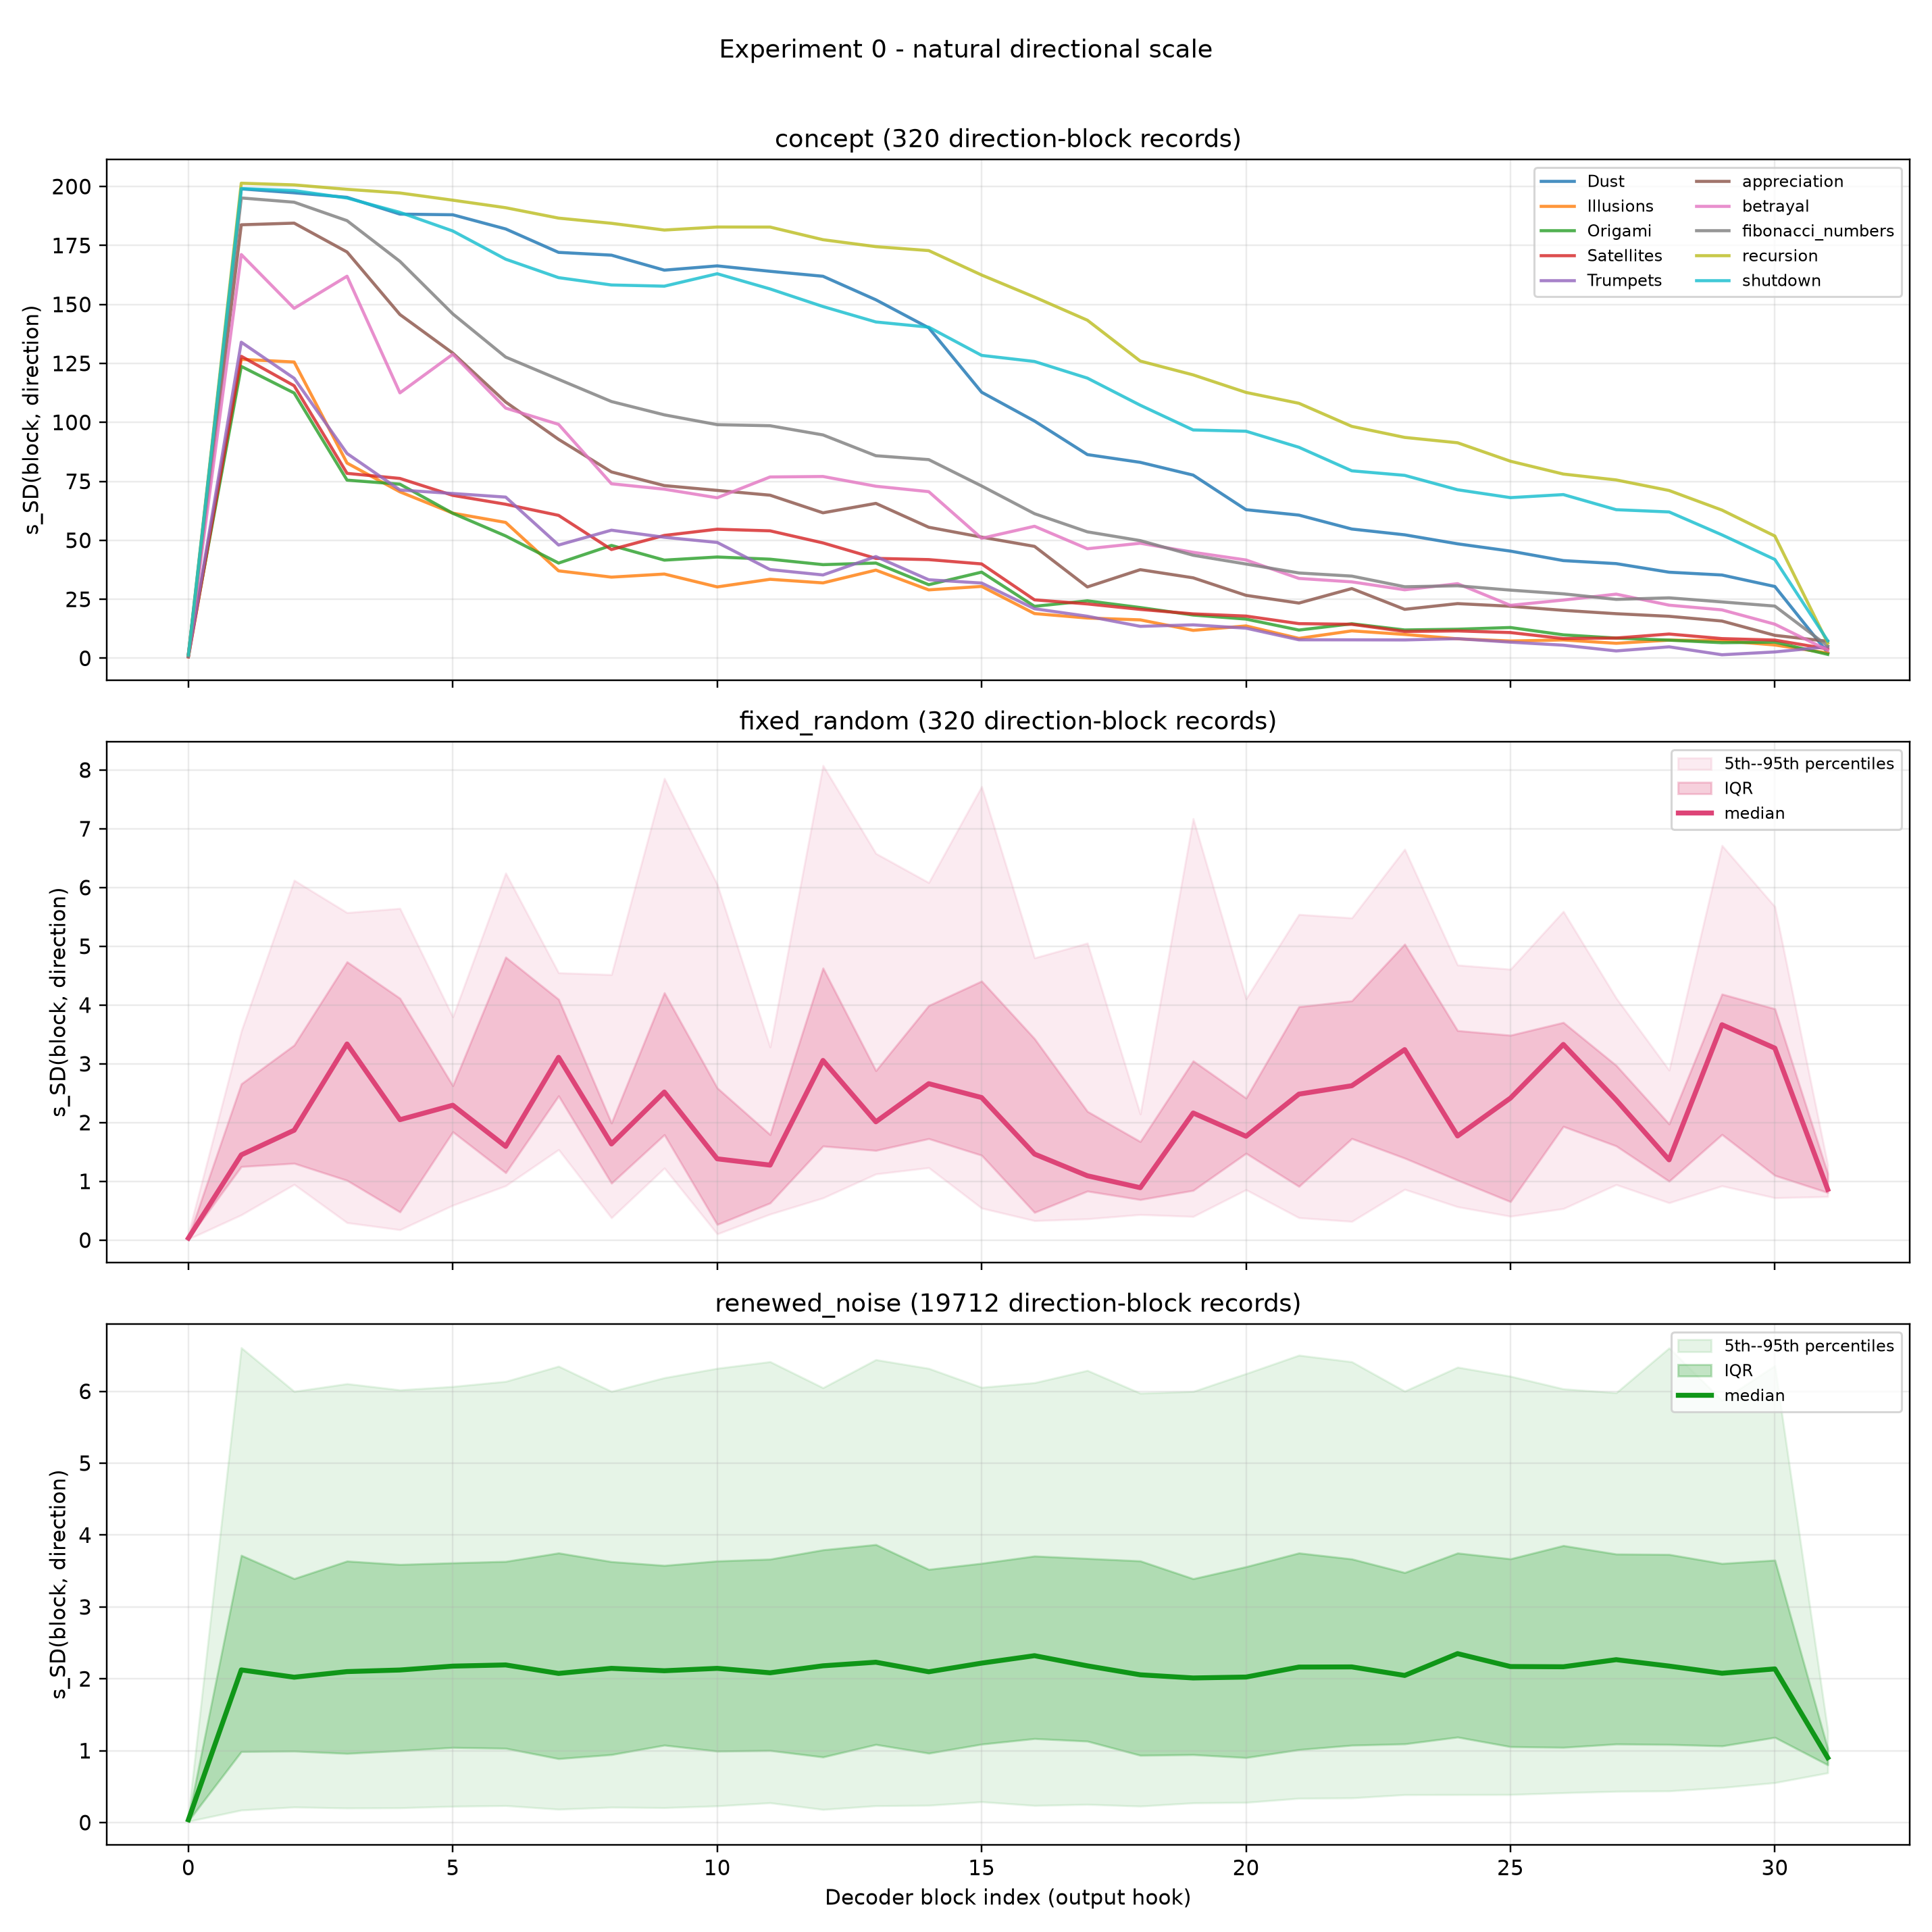
\includegraphics[width=\columnwidth]
{figures/experiment_0_scales_sd.png}
\caption{Natural directional scales across decoder blocks. Concept
directions are shown individually; isotropic controls are summarized by
their median, interquartile range, and 5th--95th percentiles.}
\label{fig:scales}
\end{figure}

Since every direction is normalized to unit norm, the directional variance
satisfies
\begin{equation}
s_{\mathrm{SD}}^2(\ell,v)
=
v^{\top}\widehat{\Sigma}_{\ell}v,
\label{eq:directional-variance}
\end{equation}
where $\widehat{\Sigma}_{\ell}$ is the empirical covariance of the
unperturbed activations at block $\ell$. The observed differences therefore
reflect how each direction is oriented relative to the activation
covariance, rather than differences in vector length. Concept directions
are more strongly aligned with high-variance axes, particularly in early
and intermediate blocks. This remains a geometric result: lexical,
positional, or construction-related components may contribute to this
alignment, so the additional variance cannot be interpreted as exclusively
semantic.

SD and corrected MAD differ markedly in internal layers. At block~1, the
median SD-to-MAD ratio is approximately 2,355 for concept directions,
compared with 51 for fixed random directions and 76 for renewed noise; the
three ratios approach one near the final block. Thus, the large SD values
do not reflect a uniform widening of the projection distributions and may
instead be driven by distinct token groups, multimodality, or distant
observations. The sentence-level bootstrap nevertheless gives a median
coefficient of variation of approximately 0.8\%, indicating that the SD
pattern is reproducible under resampling and is not attributable to a small
number of sentences.

These calibration results motivate two complementary comparisons in the
following behavioral experiments. Matching $\alpha$ preserves the absolute
size of the intervention, whereas matching
$z=\alpha/s(\ell,v)$ controls its magnitude relative to the natural
variability of the corresponding layer and direction. Because SD and MAD
capture different aspects of that variability, the latter is retained as
an alternative parameterization rather than treated only as an uncertainty
estimate. Scales must also be computed in the presentation context and at
the token positions used by each behavioral protocol. The calibration
therefore defines the measurement scale for the subsequent 2AFC experiments;
by itself, it provides no behavioral evidence of perturbation detection.

\subsection{Localization Is Confined to Early Blocks and Ordered by Threshold}
\label{sec:localization}

Llama emits the same answer label in 98.0\% of perturbed trials and its raw
accuracy stays at 0.5088 across every block and dose, its sham margin of
1.725 logits being roughly four times the effect. Sham subtraction does not
repair the readout: sham-subtracted accuracy reaches 0.5515 overall, but
0.481 when the perturbed sentence carries the first answer label against
0.753 when it carries the second, while the two physical positions stay at
0.6178 and 0.6164. The paired contrast of \cref{eq:paired} removes this
asymmetry, against a permutation null of $-0.0001\pm0.0042$ for an observed
$+0.3877$ on Llama and $+0.0002\pm0.0013$ for $+0.0554$ on Qwen; the
full bias decomposition is in \cref{app:loc-bias}. Qwen's sham
margin is 0.256 logits and its decision does move, reaching 1.000 accuracy in
all 160 trials of the concept cell at block~3 and $\alpha=16$, with a raw
threshold at $\alpha=6.26$. The two models therefore separate what a
perturbation leaves in the model from what its discrete report exposes, the
split \citet{ferrara2026} describe.

% NOTE: the point estimates below are regenerated from the completed 10x10 Llama
% panel (panel-concepts + panel-random) and reproduce exactly. The hierarchical
% intervals in the caption do NOT: no script in the repo computes them, and a
% two-stage bootstrap (resample directions, then pairs within each, 2000 draws)
% does not reproduce the previously published intervals on the OLD data either --
% it gives [0.172,0.401] where the paper had [0.225,0.381] for concept. The
% intervals below therefore come from that two-stage bootstrap, not from whatever
% produced the originals. Regenerate them with the original procedure before
% submission.
\begin{table}[H]
\centering
\small
\begin{tabular}{llrrrr}
\toprule
Model & Rule & concept & random & noise & dropout \\
\midrule
Llama & $\alpha$ & 0.317 & 0.253 & 0.294 & 0.287 \\
Llama & $z$      & 0.268 & 0.183 & 0.213 & 0.213 \\
Qwen  & $\alpha$ & 0.124 & 0.056 & 0.043 & 0.042 \\
Qwen  & $z$      & 0.137 & 0.069 & 0.057 & 0.068 \\
\bottomrule
\end{tabular}
\caption{Paired contrast $S$ by perturbation family, pooled over the
responsive blocks (Llama 0--13, Qwen 3--16). The Llama rows use ten concept
and ten fixed random directions; Qwen uses four and three. Hierarchical 95\%
intervals on the Llama $\alpha$ row, resampling directions then sentence
pairs, are $[0.239,0.388]$, $[0.227,0.281]$, $[0.253,0.334]$ and
$[0.251,0.325]$ in column order: all exclude zero, and all overlap.}
\label{tab:localization}
\end{table}

The four families order as concept, then renewed noise and dropout, then
fixed random, on both models and under both dose rules
(\cref{tab:localization}). The ordering is one of threshold rather than of
kind. At matched amplitude the Llama families overlap, with renewed noise and
dropout indistinguishable at 0.294 and 0.287, so detectability follows
amplitude and per-token renewal rather than the additive or multiplicative
form of the intervention. \Cref{fig:localization-curves} shows every family
crossing 75\% at Qwen's block~3 and then declining, with thresholds at
$\alpha=6.5$, a bracket in $[8,16]$, 63.0 and 32.3 and peak accuracies of
0.994, 0.950, 0.912 and 0.794. A concept direction needs a quarter to a tenth
of the amplitude a generic one needs, and no family is undetectable, which
agrees with the localization of dropout and Gaussian noise reported by
\citet{fornasiere2026}. The scrambled control separates orientation from
magnitude: pooled over doses, a concept direction leads its own coordinate
permutation by $1.75\times$ at block~3 and $4.19\times$ at block~6, while the
permutation falls back onto the fixed-random family, and it also collapses
the calibrated scale of a concept direction onto the fixed-random value
(\cref{app:loc-scramble}).

Localization is also confined to the early stack
(\cref{fig:localization-maps}). Llama responds in blocks 0--13 and sits
exactly at chance in blocks 14--30, at 0.4993 over 164,560 trials with ties
excluded and no family beyond $1.6\sigma$. The perturbation has not faded
there: its magnitude decays smoothly, 1.60 at block~0, 0.86 at block~13,
0.52 at block~14 and 0.06 at block~30, while accuracy falls from 0.77 to
chance in a single block. What ends at the cut is the information about which
sentence was perturbed, and \cref{sec:degradation} finds the same cut in a
task the model performs under the same perturbations. The final blocks are a structural zero, since the
intervention enters a block output at sentence positions, attention is
causal, and beyond the last block only the final normalization and the
unembedding remain, both acting position by position; Llama's block~31 ties
at every dose including a realized amplitude of 127, and Qwen's block~56
stays between 0.487 and 0.519 up to $\alpha=1024$. Qwen decays instead of
stopping, halving about every five blocks. The two models respond through the
first 44\% and the first 25\% of their stacks respectively, so relative depth
does not transfer between architectures. \Cref{app:loc-depth} gives the
per-block values under both dose rules.

Standardized matching changes the spacing of the family thresholds, not which
families respond, provided the scale is estimated in the context the task uses
and the grid reaches each family's own threshold. Re-estimating $s(\ell,v)$
inside the forced-choice prompt drops the Llama concept-to-random scale ratio
from 22.7--122 to 1.5--3.0, whereas on Qwen the ratio survives at 3.9--12.6
and a coordinate permutation collapses it onto the fixed-random value, so
there it measures alignment with the high-variance directions whose geometry
\citet{nguyen2026} model. \Cref{app:loc-scale} gives both estimates, the token that drives the
difference, and the rule used to size each grid.

Three limits bound these results, quantified in
\cref{app:loc-thresholds,app:loc-contamination}.
Only 17 of 508 fitted Llama curves give a threshold both bracketed and
interior to the tested range, so no 75\% threshold from that model should be
quoted. Relabeling the two options, with the same sentences, order and
perturbation, changes Llama's $S$ by a factor of 2.4 while physical order
stays balanced. Leakage from the targeted sentence to the other saturates on
Llama, so at the top of the grid the second sentence is no longer an intact
control. Finally, the answer tracks which sentence was perturbed, and nothing
here separates a report about an internal state from a discrimination driven
by the downstream effects of the perturbed tokens, the distinction
\citet{singh2026} require.

\begin{figure}[H]
\centering
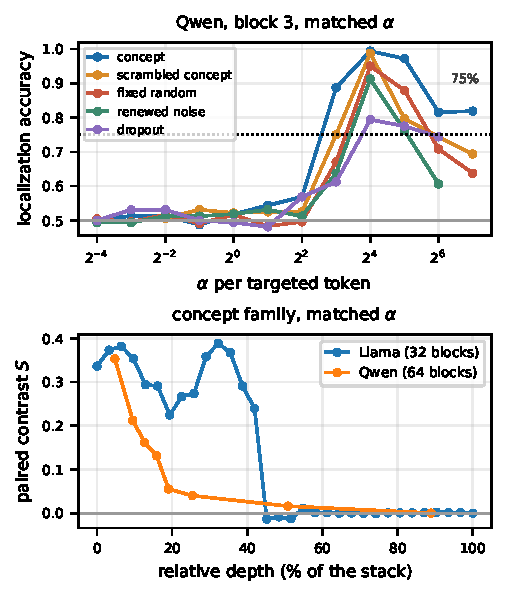
\includegraphics[width=\columnwidth]{figures/localization_curves.pdf}
\caption{Top: localization accuracy against raw amplitude at Qwen's block~3,
with the 75\% criterion dotted. Every family crosses it and every family
declines above $\alpha=16$, so the families separate by threshold and the
monotone psychometric form fails at the top of the grid. The scrambled
concept, a coordinate permutation of a concept vector, falls between concept
and the isotropic families. Bottom: paired contrast against relative depth,
concept family. Llama stops abruptly near 44\% of its stack while Qwen decays
from the start, so the responsive band is not a fixed fraction of depth.}
\label{fig:localization-curves}
\end{figure}

\subsection{Detection Without a Broken Model}
\label{sec:degradation}

A perturbation large enough to be located might simply be large enough to
break the model, in which case \cref{sec:localization} measures damage rather
than access. We therefore ran the same interventions under a task that never
mentions them: the model reads one sentence and answers whether it expresses a
queried concept, never the injected one (\cref{sec:degradation-approach}).
Each of the 436,480 perturbed trials is paired with a localization cell at the
same block, family and dose. Undisturbed, the model answers 0.819 of these
correctly against a floor of 0.5, so there is room to fall.

Damage stops where localization stops (\cref{fig:degradation-depth}). Pooled
over the four largest amplitudes, the contiguous band of blocks in which some
family loses at least 5 points runs from 0 to 13, for any threshold between 2
and 5 points, and blocks 0--13 are also the responsive band of
\cref{sec:localization}, found on a different task, prompt and corpus. Inside
the band a concept direction breaks the task about five blocks deeper than any
control, which we cannot yet credit to its content, since those directions
carry the position-0 component of \cref{app:loc-scale}.

Damage and detection mostly rise together, correlating at $-0.72$ for concept
through $-0.50$ for fixed random directions, so disruption explains most of
the design but not all of it. Of the 1,240 cells matched on raw amplitude, 30
are located at 70\% or better while classification stays within 5 points of
sham, and in the concept family these form one connected block of cells at
blocks 9--13 and moderate amplitude (\cref{fig:degradation-regimes}), where
the paired contrast averages 0.331 against 0.317 for the responsive band as a
whole. Detection can therefore happen with the task intact, over a narrow part
of the design, but the margin over the band is slight, and it says nothing
about whether the mechanism is introspective. At matched damage a concept direction is no more detectable
than a random one (\cref{tab:app-deg-matched}), the conclusion the scrambled
control of \cref{sec:localization} reaches by another route. \Cref{app:degradation} gives the limits,
one of which voids the standardized half of this sweep.

\begin{figure}[H]
\centering
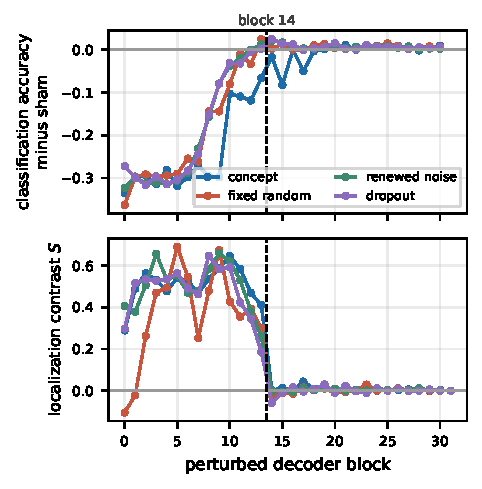
\includegraphics[width=\columnwidth]{figures/degradation_depth.pdf}
\caption{Both measures by perturbed block on Llama, pooled over the four
largest raw amplitudes. Top: accuracy lost on the semantic task against sham.
Bottom: the localization contrast of \cref{eq:paired} on the same
amplitudes. Both collapse at the same block, marked by the dashed rule, on
tasks that share nothing but the intervention.}
\label{fig:degradation-depth}
\end{figure}

\subsection{Multi-injection highlights the model's biases}

\label{sec:multi-injection-results}

Across counting, identification, and ordering (\cref{sec:multi-injection-approach}), the dominant finding is a strong, content-independent default-answer bias, not tracking of injection count, identity, or relative depth.
\Cref{tab:multi-injection-summary} summarizes the headline statistics; full per-dose numbers and the modulator sweeps are in \cref{app:multi-injection}.

\paragraph{Counting.}
At the true sham ($k{=}0$), the model answered ``1'' in 100\% of trials across both dosing regimes and every tested $\alpha$, never once answering ``0''; the response distribution stays concentrated on ``0''/``1'' regardless of the true count (\cref{fig:e9-dist}).
A bias-adjusted digit-logit contrast, $\mathrm{logit}(k)-\mathrm{logit}(\text{``1''})$, rules out a decoding-only account: it is strongly and consistently \emph{negative} at every dose (\cref{fig:e9-logit})---the raw logits themselves prefer ``1'' over the true count ($-1.81$ pooled, $t=-34.7$, $p=1.8\times10^{-186}$, $n=1{,}280$).

\paragraph{Identification.}
Forced-choice exact match (both slots correct) is 0.0--1.2\% in every condition, including \texttt{single\_concept} where only one slot names a specific concept; free-response similarity to the truly injected concept clears threshold in 2.8--4.7\% of trials (\cref{fig:e10}).
The one clean positive control is the sham condition's false-identification rate, exactly 0\%.

\paragraph{Relative-depth ordering.}
Raw accuracy is 53.0\%, not distinguishable from chance ($p=0.25$), and decomposes into a strong response-position bias: 94.9\% accuracy when the correct concept happened to be labeled \texttt{A}, 11.2\% when labeled \texttt{B}.
A bias-adjusted logit contrast initially suggested a small residual signal (mean $+0.38$ at $\alpha{=}2\text{--}3$, $t=1.28$, $p=0.20$), but the paired-sham control shows this was the prompt's own baseline preference: sham trials (zero injection, identical prompt) produce an almost identical contrast ($+0.258$) to injected trials ($+0.272$), leaving a double-adjusted, injection-specific contrast of $+0.014$ ($p=0.91$, $n=480$; \cref{fig:e11-sham}).

\paragraph{Modulators.}
Sweeping ordering against layer distance (E4) reproduces a positive, now nominally significant contrast ($+0.322$, $t=3.43$, $p=0.0006$, $n=1{,}680$) of the same sign and similar magnitude to ordering's own pre-sham result; given that result's fate above, E4 should be read as unconfirmed pending the same paired-sham test, not as established.
Dose ratio (E5) and concept similarity (E6) both show large apparent effects that fully decompose into the same \texttt{A}-bias once split by which letter was actually correct (\cref{fig:modulators-bias,app:multi-injection}), and E5's raw-accuracy trend is additionally confounded with dose magnitude exceeding the validated coherence range.

These results converge with the response-bias controls proposed in \cref{sec:proposal}: a discrete report can be dominated by a default answer that survives coherence filtering and, for counting, is present in the raw logits themselves---underscoring why localization and presence judgments alone cannot establish that a report tracks the manipulated factor.

\begin{table}[H]
\centering
\small
\begin{tabular}{lll}
\toprule
Experiment & Metric & Result \\
\midrule
Counting & $P(\text{``1''}\mid k{=}0)$ & 100\% \\
Counting & logit$(k)-$logit(``1'') & $-1.81$ \\
Identification & forced-choice exact match & 0.0--1.2\% \\
Ordering & raw accuracy & 53.0\% \\
Ordering & double-adj.\ contrast & $+0.014$ \\
\bottomrule
\end{tabular}
\caption{Headline null results across the multi-injection tasks. Full statistics, sample sizes, and $p$-values are given in the text and \cref{app:multi-injection}.}
\label{tab:multi-injection-summary}
\end{table}

\begin{figure}[H]
\centering
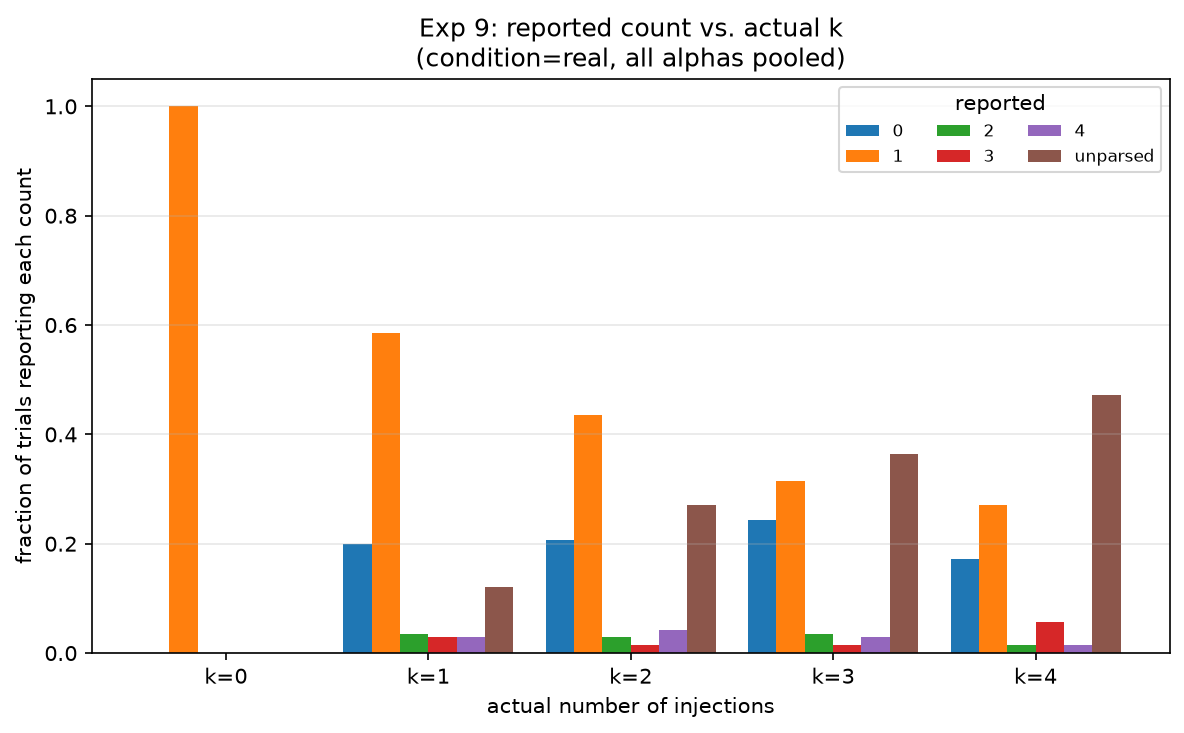
\includegraphics[width=\columnwidth]{figures/e9_response_distribution.png}
\caption{Reported count vs.\ true $k$: responses stay concentrated on ``0''/``1'' regardless of $k$.}
\label{fig:e9-dist}
\end{figure}

\begin{figure}[H]
\centering
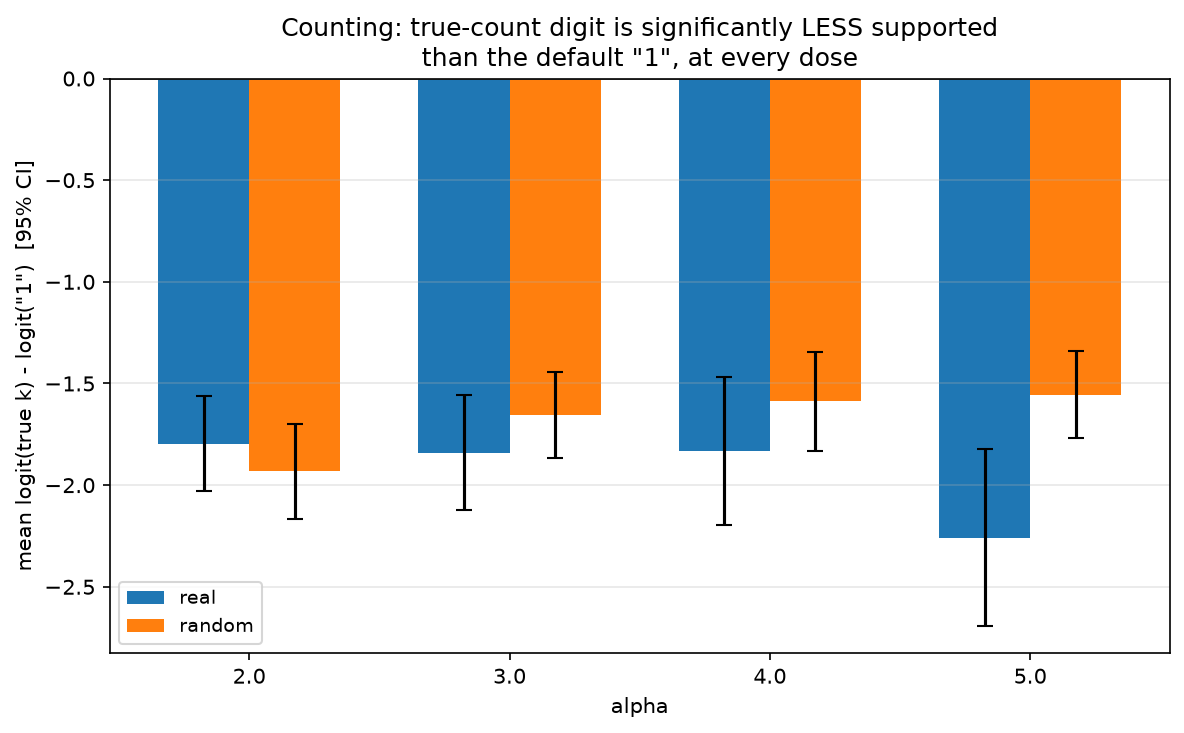
\includegraphics[width=\columnwidth]{figures/summary_counting_digit_logit_contrast.png}
\caption{Digit-level logit contrast $\mathrm{logit}(k)-\mathrm{logit}(\text{``1''})$, negative at every tested dose.}
\label{fig:e9-logit}
\end{figure}

\begin{figure}[H]
\centering
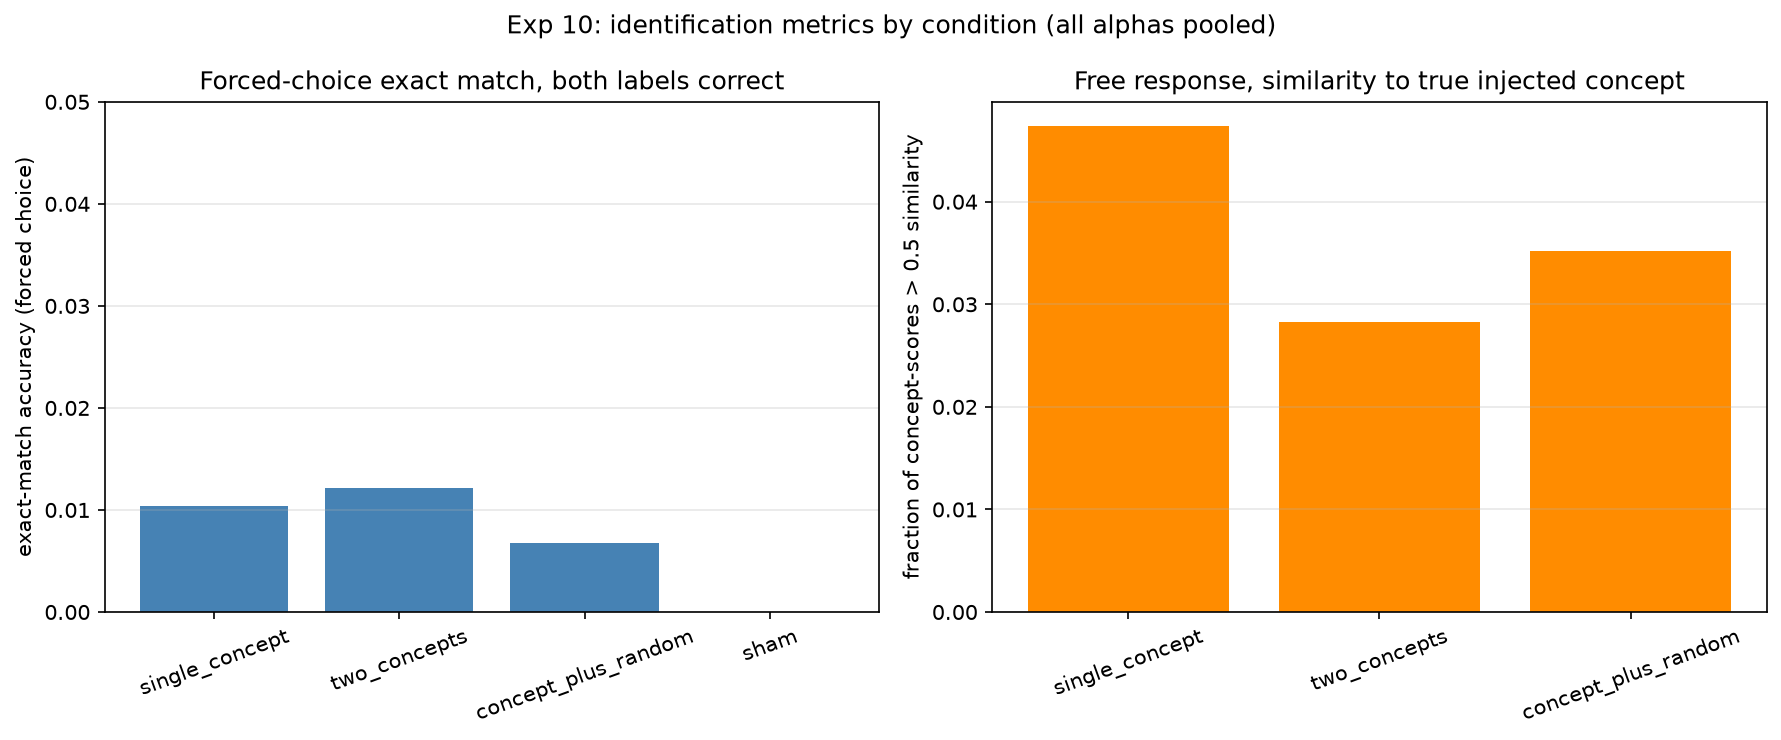
\includegraphics[width=\columnwidth]{figures/e10_metrics_by_condition.png}
\caption{Identification metrics by condition: forced-choice and free-response accuracy remain near floor throughout.}
\label{fig:e10}
\end{figure}

\begin{figure}[H]
\centering
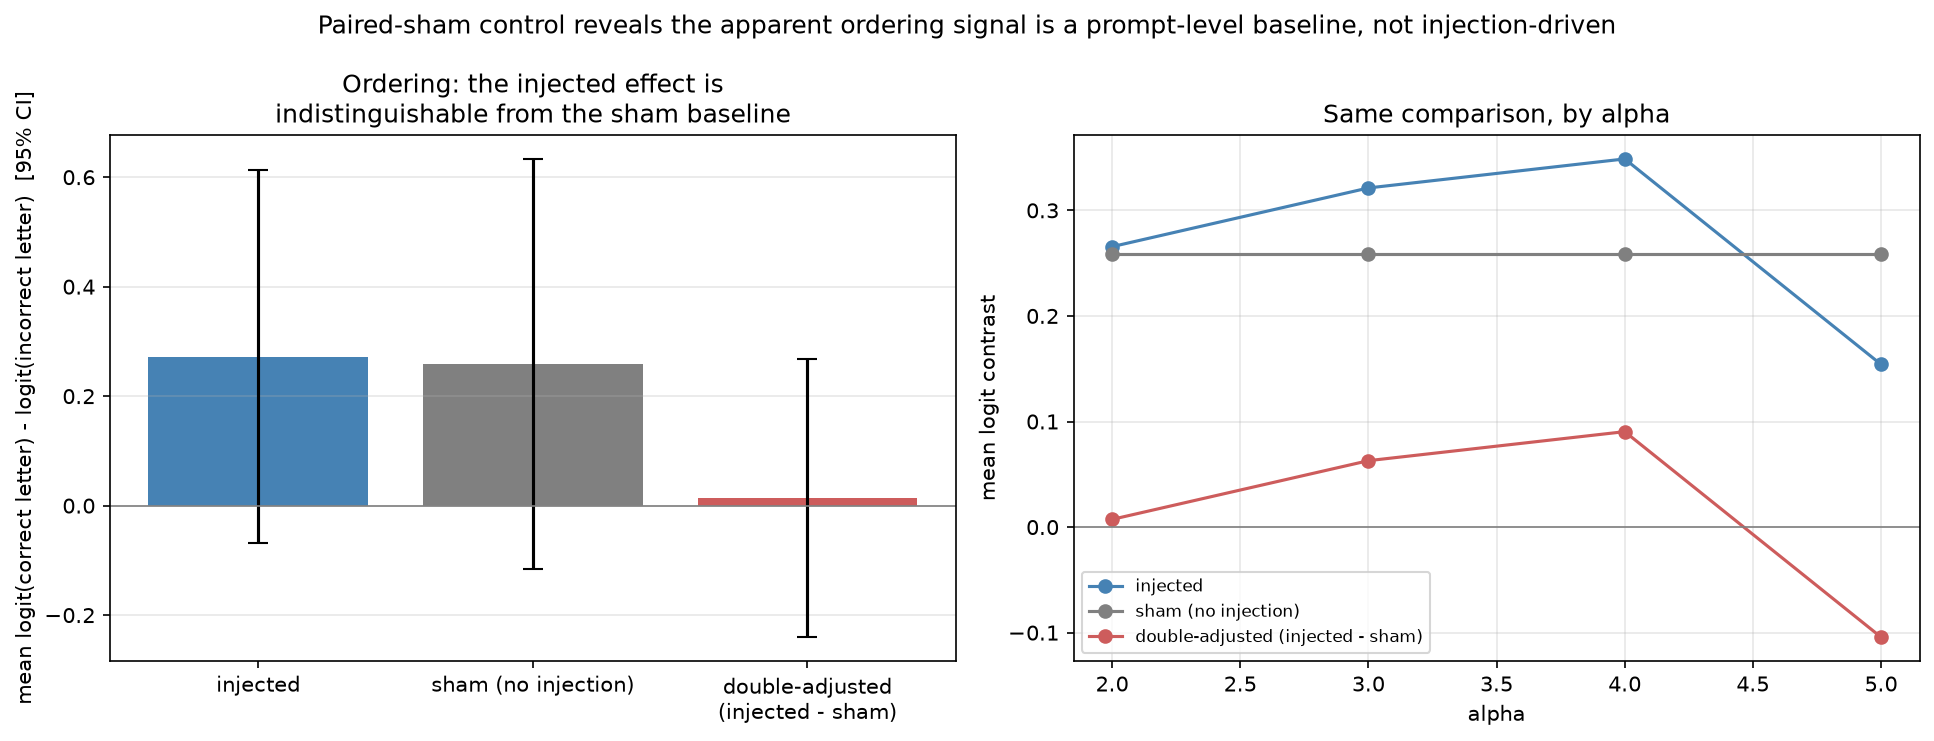
\includegraphics[width=\columnwidth]{figures/summary_ordering_sham_reveal.png}
\caption{Ordering: injected and paired-sham logit contrasts track each other closely; the double-adjusted, injection-specific contrast is flat around zero.}
\label{fig:e11-sham}
\end{figure}

\begin{figure*}[t]
\centering
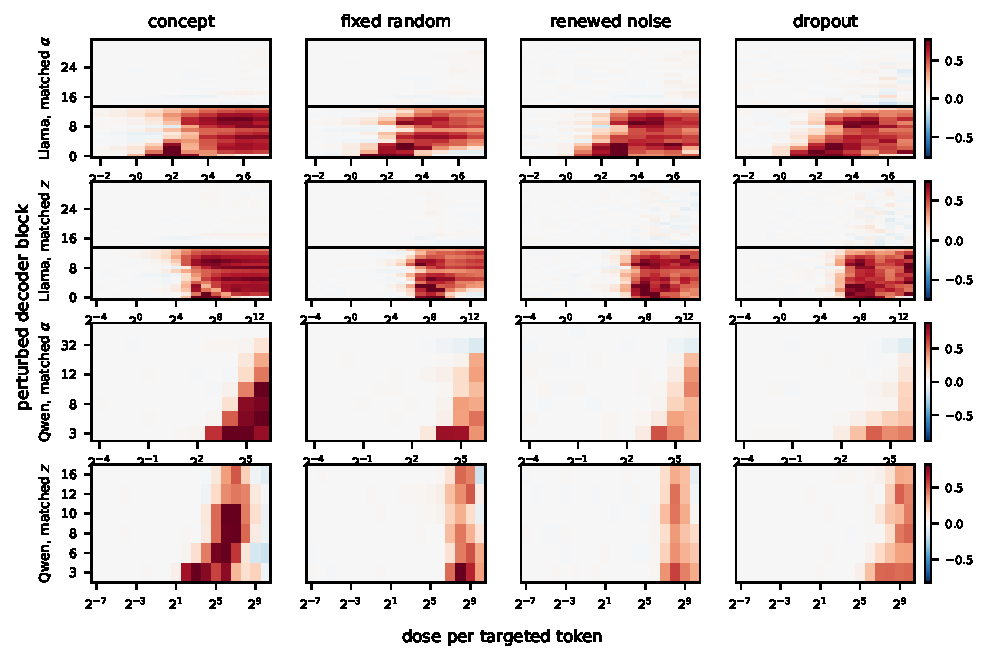
\includegraphics[width=0.95\textwidth]{figures/localization_maps.pdf}
\caption{Mean paired contrast $S$ by perturbed block and dose, one column per
perturbation family, one row per model and dose rule, each row on its own
colour scale. Standardized rows divide by scales estimated in the
forced-choice context. The rule marks Llama's block~14, above which every
cell is neutral at every dose, including doses that deliver four orders of
magnitude more raw amplitude than the responsive blocks require. The concept
front lies left of the three control fronts in all four rows, and concept
fades at the top of its range while the controls are still rising.}
\label{fig:localization-maps}
\end{figure*}

\bibliography{article-references}
\bibliographystyle{icml2025}

\newpage
\onecolumn
\appendix
% Appendix for the forced-choice localization results of \cref{sec:localization}.
% Input from results.tex, after \appendix and before the multi-injection appendix,
% so that the appendix order follows the order of the Results section.

\section{Localization: Additional Details}
\label{app:localization}

\subsection{Sweeps}
\label{app:loc-design}

Every sweep uses the same material: five sentence pairs matched for token
length, concept directions, fixed random directions, and two renewed-noise and
two dropout realizations per block. Llama uses the ten concepts of the
repository (\emph{Dust}, \emph{Satellites}, \emph{Trumpets}, \emph{Origami},
\emph{Illusions}, \emph{appreciation}, \emph{betrayal},
\emph{fibonacci\_numbers}, \emph{recursion}, \emph{shutdown}) and ten fixed
random directions, matching the number of conceptual directions. Qwen was not
extended and keeps four concepts (\emph{Dust}, \emph{Satellites},
\emph{recursion}, \emph{shutdown}) and three fixed random directions, so its
family means rest on a narrower and less representative panel. Each cell is run in both
physical orders and under both label assignments, for 20 sham conditions per
model. Each model was swept twice, once under raw amplitude and once under
standardized dose (\cref{tab:app-loc-trials}).

\begin{table}[H]
\centering
\small
\begin{tabular}{llrr}
\toprule
Model & Rule & Dose grid & Trials \\
\midrule
Llama & $\alpha$ & $0.25$--$128$, 10 doses & 306,280 \\
Llama & $z$ & $0.0625$--$8192$, 18 doses & 253,460 \\
Qwen & $\alpha$ & $0.0625$--$64$, 11 doses & 79,700 \\
Qwen & $z$ & $0.0078$--$1024$, 18 doses & 47,540 \\
\bottomrule
\end{tabular}
\caption{Dose grids and trial counts. Llama covers all 32 decoder blocks;
Qwen covers blocks 3, 6, 8, 10, 12, 16, 32 and 56 of 64 under raw amplitude
and the six responsive blocks under standardized dose. The two control runs
add 17,620 trials at the deepest Qwen blocks and 37,000 trials for the
scrambled-concept family. Two panel-completion runs add a further 465,960
trials, carrying Llama to ten concepts and ten fixed random directions on both
rules over all 32 blocks; the concept family is absent from block 31 under raw
amplitude, which the depth analyses therefore read over blocks 0--30.}
\label{tab:app-loc-trials}
\end{table}

\subsection{Response Bias and the Paired Estimator}
\label{app:loc-bias}

Llama prefers the letter \texttt{A} in all 20 sham conditions, by $+1.725$
logits, and a perturbation moves that by about a quarter, never enough to flip
the answer. Subtracting the sham does not fix the readout, because the bias is
uneven: sham-subtracted accuracy is 0.481 when the perturbed sentence is
labeled \texttt{A} and 0.753 when it is labeled \texttt{B}, while the two
physical positions give 0.6178 and 0.6164. Perturbing either sentence pushes
the logits away from the default answer, by $-0.310$ on average, which scores
as a success whenever the target carries the other label. The paired contrast
removes it: permuting which sentence was the target, every logit unchanged,
gives $-0.0001\pm0.0042$ over 200 draws against an observed $+0.3877$ on
Llama, and $+0.0002\pm0.0013$ against $+0.0554$ on Qwen.

Llama answers with something other than a letter in 0.83\% of trials and 5.4\%
at $\alpha=128$, mostly in the concept family; Qwen does so in 53\% including
sham, and less often as the dose grows, so that rate comes from its chat
template and leaves the logit readout alone. Ties from the bfloat16 step of
about $0.0625$ cover 41.4\% of Llama trials, 55\% in the dead blocks against
20\% in the live ones, so the depth analysis drops them.

\subsection{Depth Profile}
\label{app:loc-depth}

The cut between blocks 13 and 14 is there under both dose rules
(\cref{tab:app-loc-depth}). The standardized grid delivers up to a thousand
times more raw amplitude at the deep blocks than the live blocks need, so the
deep zero is not a coverage problem: the best deep cell of any family reaches
0.61 against 0.70 to 0.92 in the live blocks, and block 31 returns exactly
0.500 at all 18 doses.

\begin{table}[H]
\centering
\small
\begin{tabular}{llrr}
\toprule
Model & Block & $\alpha$-matched & $z$-matched \\
\midrule
Llama & 3  & 0.306 & 0.250 \\
      & 6  & 0.245 & 0.253 \\
      & 10 & 0.369 & 0.347 \\
      & 13 & 0.235 & 0.235 \\
      & 14 & $-$0.001 & 0.007 \\
      & 16 & $-$0.004 & 0.001 \\
      & 31 & --- & 0.000 \\
\midrule
Qwen  & 3  & 0.353 & 0.236 \\
      & 6  & 0.212 & 0.148 \\
      & 10 & 0.131 & 0.155 \\
      & 12 & 0.055 & 0.079 \\
      & 16 & 0.040 & 0.057 \\
      & 32 & 0.016 & --- \\
      & 56 & 0.000 & --- \\
\bottomrule
\end{tabular}
\caption{Concept-family paired contrast $S$ by block. The concept direction
failed its norm check at Llama's block 31 under raw amplitude, and the Qwen
standardized sweep covers the responsive blocks only.}
\label{tab:app-loc-depth}
\end{table}

\Cref{fig:app-maps} enlarges \cref{fig:localization-maps} one model at a time.

\begin{figure}[htbp]
\centering
\begin{minipage}[t]{0.48\textwidth}
\centering
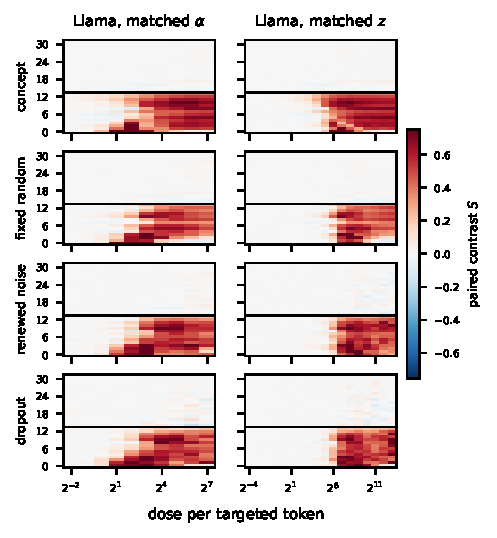
\includegraphics[width=\linewidth]{figures/localization_maps_llama.pdf}
\end{minipage}\hfill
\begin{minipage}[t]{0.48\textwidth}
\centering
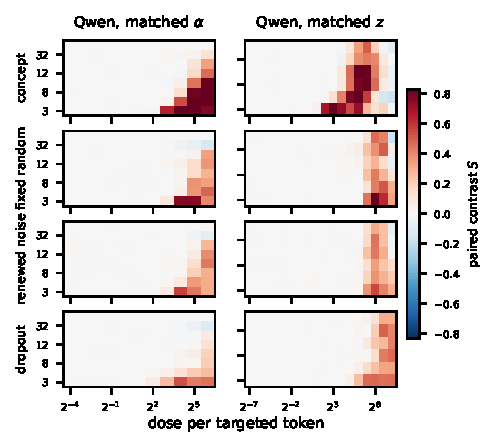
\includegraphics[width=\linewidth]{figures/localization_maps_qwen.pdf}
\end{minipage}
\caption{Paired contrast $S$ on Llama (left) and Qwen (right), one row per
perturbation family and one column per dose rule, with the perturbed block on
the vertical axis and the dose on the horizontal one. Above Llama's rule at
block 14 every cell is neutral at every dose, including standardized doses
that deliver orders of magnitude more raw amplitude than the responsive blocks
require. Qwen decays with depth instead of stopping, and its standardized
column covers the responsive blocks only.}
\label{fig:app-maps}
\end{figure}

\subsection{Where the Scale Is Estimated}
\label{app:loc-scale}

A sentence rendered on its own starts at position 0, where Llama's activation
has norm near 547 against 1.7 to 9.7 everywhere else, and that token is 16\%
of the calibration sample; one concept direction at block 1 projects 582.3
onto it and 0.399 onto every other position. The forced-choice prompt puts the
perturbed tokens at positions 57 to 75, so that token never appears. Concept
vectors are averages of hidden states and inherit the component: their cosine
with the mean position-0 activation runs 0.21 to 0.99, against 0.001 to 0.035
for random directions, which reproduces the measured scale ratio. Qwen does
not do this, and permuting a concept vector's coordinates drops its scale from
1.227 to 0.091 at block 3, onto the fixed-random value of 0.098.
\Cref{tab:app-loc-scales} gives the ratios that dividing by $s(\ell,v)$
removes.

\begin{table}[H]
\centering
\small
\begin{tabular}{llr}
\toprule
Model & Calibration context & concept / fixed random \\
\midrule
Llama & isolated sentence & 22.7--122 \\
Llama & forced-choice prompt & 1.5--3.0 \\
Qwen  & isolated sentence & 5.8--15.8 \\
Qwen  & forced-choice prompt & 3.9--12.6 \\
\bottomrule
\end{tabular}
\caption{Ratio of the median concept scale to the median fixed-random scale,
over the responsive blocks of each model.}
\label{tab:app-loc-scales}
\end{table}

The grid must also reach each family's own threshold, which in $z$ is its
threshold in $\alpha$ divided by its scale: a grid chosen without looking at
the scales reaches one family's transition and not another's, and the untested
families look inert. Each standardized grid here is sized so that its top dose
beats, in every cell, the amplitude that family needs for 75\% correct on the
raw grid.

\subsection{Limits of the Readout}
\label{app:loc-thresholds}

\paragraph{Thresholds.} Only 17 of 508 fitted Llama curves give a threshold
both bracketed and inside the tested range, so no 75\% threshold is quoted for
that model. The curve shape is the cause, not noise: the controls peak before
the top dose and fall 0.16 to 0.21 below a monotone logistic fit, concept
saturates and falls 0.049, and Qwen peaks at $\alpha=16$ at block 3.

\paragraph{Dropout dose.} Its realized rate reaches 0.976 at $\alpha=128$, so
the top doses erase the sentence instead of raising the dose, and the realized
amplitude falls to 99.4 for 128 requested. The three additive families deliver
the request to within $5\times10^{-5}$.

\paragraph{Labels.} Relabeling the two options, with the same sentences, order
and perturbation, moves Llama's $S$ from 0.379 to 0.160 and Qwen's from 0.0593
to 0.0515.

\phantomsection\label{app:loc-contamination}
\paragraph{Leakage.} Leakage from the perturbed sentence to the other
saturates on Llama within two blocks and never decays, with several cells
above 1.0. Attention is causal, so it runs one way and no balancing of trials
repairs it. On Qwen its median is 0.067.

\phantomsection\label{app:loc-scramble}
\paragraph{Scrambled concept.} A concept direction beats its own coordinate
permutation $1.75\times$ at block 3, $+0.445$ against $+0.255$, and
$4.19\times$ at block 6, $+0.300$ against $+0.072$, while the permutation sits
with fixed random at $+0.228$ and $+0.128$. Orientation, not coordinate
statistics, carries the advantage.

\paragraph{Two unexplained results.} Thirteen cells of 2794 sit significantly
below chance, all fixed random, all at Llama's blocks 7 and 12, under both
dose rules. At Qwen's block 32 the families split by sign, concept at $+0.016$
against $-0.013$ to $-0.022$; content does not explain that split, since a
permuted concept vector carries none and still gives the positive sign,
$+0.022$ against $-0.027$. What concept and its permutation share is
heavy-tailed coordinates, kurtosis 6 to 8.5 against 3.

% Appendix for the semantic control task of \cref{sec:degradation}.
% Input from results.tex, after the localization appendix, so that the appendix
% order follows the order of the Results section.
% Source: results/experiment4/main/summary.json, the per-cell summary of Slurm
% job 8333, joined cell by cell against results/experiment1/full32_all.
% Figures: python code/analysis/plot_paper_figures.py

\section{Task Degradation: Additional Details}
\label{app:degradation}

\subsection{Sweep}
\label{app:deg-design}

% CONSISTENCY NOTE (2026-09-16). Experiment 1 was extended to ten concept and ten
% fixed random directions; this sweep was not, and it imports nothing from it
% (summary.json has experiment1_summary: null -- its detection_accuracy is measured
% here). So no number below is arithmetically stale. Two mismatches remain, both
% understating this sweep's concept row relative to Experiment 1:
%   1. It injects only Dust and Satellites, and Dust carries 3 of the 5 evaluated
%      concepts, i.e. 60% of the concept cells. Dust is 9th of 10 in Experiment 1's
%      alpha panel (S = +0.059 against a panel mean of +0.143), so this sweep's
%      concept axis sits about 33% below the full panel's concept mean.
%   2. Detection here is adjusted accuracy at a 0.70 threshold, the estimator
%      app:loc-bias shows does not remove the answer bias; Experiment 1 reports the
%      paired contrast S for that reason. Mean detection accuracy is 0.536-0.569
%      across families, i.e. the bias-pinned regime.
% Also: this sweep's calibration is the superseded isolated-sentence one and its z
% grid stops at 20.48, so its standardized half is void -- already stated below, and
% every figure filters to matched alpha.
Five concepts of the complex-example corpus are evaluated
(\emph{appreciation}, \emph{betrayal}, \emph{Fibonacci numbers},
\emph{recursion}, \emph{shutdown}), each with four positive and four negative
sentences under both assignments of the letters \texttt{X} and \texttt{Y}: 80
items over 40 distinct sentences. The injected direction, \emph{Dust} or
\emph{Satellites}, is never the evaluated concept. The sweep covers blocks
0--30, the four families, ten raw amplitudes from $0.25$ to $128$ and twelve
standardized doses, for 436,480 perturbed trials against the same 80 sham
trials throughout, with 80 trials per concept cell, 160 for renewed noise and
for dropout and 240 for fixed random, those families carrying two, two, two
and three directions or realizations. Block 31 is excluded: its concept
directions cannot be rebuilt to the norm the calibration recorded, and by
\cref{sec:localization} it is structurally dead in any case.

\subsection{Depth Profile and Matched Degradation}
\label{app:deg-depth}

Blocks 0--7 do not separate the families (\cref{tab:app-deg-depth}): in the
early stack everything breaks the task equally, between $-0.23$ and $-0.36$.
From block 8 the three controls recover and the concept family does not, the
gap peaking at $-0.197$ at block 9: the deepest block whose pooled loss still
reaches 5 points is 9 for renewed noise and for dropout, 10 for fixed random
directions and 15 for concept. Above the contiguous band the concept family
oscillates rather than staying flat, $-0.083$ at block 15 against $0.000$ at
block 16, so isolated deep cells survive that criterion while
\cref{sec:localization} reports the deep localization zero as exact.

\begin{table}[H]
\centering
\small
\begin{tabular}{rrrrrr}
\toprule
Block & Concept & Fixed & Noise & Dropout & Gap \\
\midrule
7  & $-0.272$ & $-0.261$ & $-0.231$ & $-0.245$ & $-0.026$ \\
8  & $-0.295$ & $-0.144$ & $-0.157$ & $-0.152$ & $-0.144$ \\
9  & $-0.298$ & $-0.144$ & $-0.079$ & $-0.080$ & $-0.197$ \\
10 & $-0.103$ & $-0.081$ & $-0.038$ & $-0.031$ & $-0.053$ \\
12 & $-0.119$ & $-0.033$ & $0.000$  & $-0.004$ & $-0.106$ \\
15 & $-0.083$ & $0.014$  & $0.017$  & $0.014$  & $-0.098$ \\
18 & $-0.003$ & $0.010$  & $0.002$  & $0.003$  & $-0.008$ \\
\bottomrule
\end{tabular}
\caption{Classification accuracy minus sham, pooled over the four largest raw
amplitudes. Fixed denotes fixed random directions. Gap is concept minus the
mean of the three controls.}
\label{tab:app-deg-depth}
\end{table}

\Cref{tab:app-deg-matched} bins the cells of both dose rules by accuracy loss
and compares localization within each bin.

\begin{table}[H]
\centering
\small
\begin{tabular}{lrrrr}
\toprule
Accuracy loss & Concept & Fixed & Noise & Dropout \\
\midrule
$[-1.00,-0.30)$ & 0.733 & 0.588 & 0.716 & 0.671 \\
$[-0.30,-0.15)$ & 0.712 & 0.659 & 0.688 & 0.693 \\
$[-0.15,-0.05)$ & 0.658 & 0.643 & 0.709 & 0.718 \\
$[-0.05,+0.05]$ & 0.521 & 0.508 & 0.518 & 0.516 \\
\bottomrule
\end{tabular}
\caption{Mean localization accuracy at matched classification loss, both dose
rules pooled. Doses are pooled inside a bin, so a family that reaches a bin at
a much lower dose than another is not distinguished here.}
\label{tab:app-deg-matched}
\end{table}

\subsection{Maps}
\label{app:deg-maps}

\begin{figure}[htbp]
\centering
\begin{minipage}[t]{0.48\textwidth}
\centering
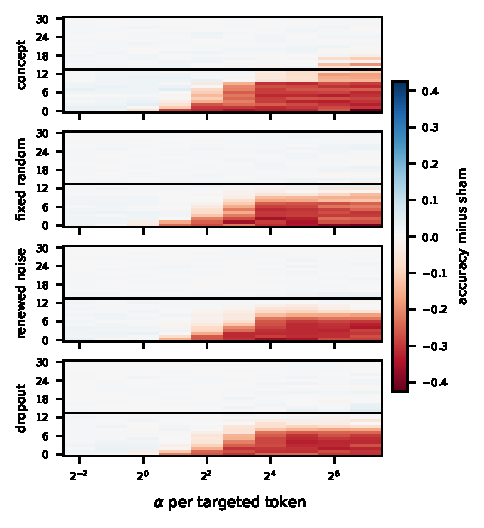
\includegraphics[width=\linewidth]{figures/degradation_maps.pdf}
\end{minipage}\hfill
\begin{minipage}[t]{0.48\textwidth}
\centering
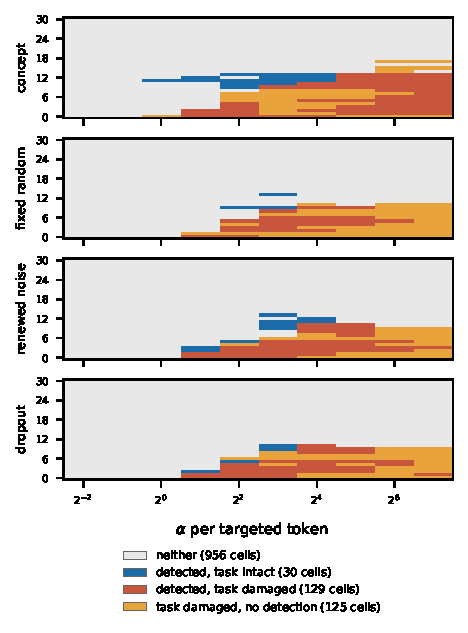
\includegraphics[width=\linewidth]{figures/degradation_regimes.pdf}
\end{minipage}
\caption{Left: classification accuracy minus sham by block and raw amplitude,
one row per family, red for degradation; the rule marks block 14, the first
block above the contiguous degraded band, and the colour scale is symmetric
about zero by construction, so that deep-block noise does not read as vividly
as shallow-block collapse. Right: the joint regimes over the same cells. A
cell counts as detected when the localization accuracy of the paired cell
reaches 70\%, and as damaged when classification accuracy falls more than 5
points below sham. Blue is the regime in which detection does not require
disruption; in the concept row those cells form a connected region over blocks
9--13.}
\label{fig:degradation-regimes}
\end{figure}

\subsection{Limits}
\label{app:deg-limits}

\paragraph{The standardized half is not a family comparison.}
Its $z$ grid was copied from the first localization sweep, so that cells would
pair exactly, and that grid divides by the isolated-sentence scales
\cref{app:loc-scale} rejects. The defect compounds: the detection side of every
standardized pairing comes from that same superseded sweep, and on the
classification side the whole active region of the three controls is
compressed into the four largest doses against the edge of the grid, so no
control is tested near its own transition. The raw-amplitude results invoke no
calibrated scale.

\paragraph{The detection side of the join is the biased metric.}
Each cell is paired with the sham-subtracted accuracy of the localization
sweep, which \cref{app:loc-bias} shows is inflated where the perturbed
sentence carries the second label, and the 70\% criterion inherits that.
Recomputing the paired contrast of \cref{eq:paired} on the 14 concept cells of
the detected-and-intact region gives a mean $S$ of 0.339 against 0.301 over
the responsive band, so that region is not an artefact of the weaker metric.

\paragraph{The concept pairing is not matched across the join.}
The per-dose table of the localization sweep pools four concept directions
where this sweep injects two, so the concept row of every pairing relates
neighboring but non-identical sets of directions. The three control families
are unaffected.

\paragraph{Output displacement, format compliance and task loss are three
quantities.}
The invalid-answer rate rises from 2.5\% at sham to 94.2\% at its worst and
fails independently of competence: at block 9 and $\alpha=8$ the concept
family has lost 15 points of accuracy while still emitting a valid letter on
97.5\% of trials. At block 9 and $\alpha=128$ its Jensen--Shannon divergence
reaches 0.600 bit against 0.040 for renewed noise, a ratio of 15, while their
accuracy losses stand at 29 and 6 points, a ratio of 5. That divergence rests
on two sampled trials per cell, three for fixed random, so it supports a median
over cells and not a cell-by-cell reading.

\paragraph{Dropout is matched only in expectation, and the items are few.}
Realized displacement tracks the request for the three additive families,
128.04, 128.00 and 128.00 at block 9 for a request of 128, and undershoots for
dropout at 112.70, whose amplitude is set through a rate. The 80 items rest on
5 evaluated concepts, 40 sentences and 2 injected directions, and reported
errors are trial-level, so between-item variability is not decomposed.


\section{Multi-Injection Experiments: Additional Details}
\label{app:multi-injection}

This appendix supplements \cref{sec:multi-injection-results} with the full experimental design, per-dose statistics, and the modulator bias decomposition referenced there.

\subsection{Design and trial counts}

\Cref{tab:multi-injection-trials} lists, for each task, the script, the manipulated conditions, and the number of trials collected in each of two experimental rounds.
Round 1 swept $\alpha\in\{1,\dots,7\}$ across all four tasks and is where the default-answer bias described in \cref{sec:multi-injection-results} was first observed.
Round 2 re-ran counting and ordering over a narrower $\alpha\in\{2,\dots,5\}$ range with the bias-adjusted logit contrast and, for ordering, the paired-sham control added; identification and the modulator sweeps were not re-run under Round 2 and so lack the sham control.

\begin{table}[H]
\centering
\small
\begin{tabular}{llrr}
\toprule
Task & Script & R1 trials & R2 trials \\
\midrule
Counting & \texttt{multi\_detection.py} & 5{,}600 & 2{,}880 \\
Identification & \texttt{multi\_identification.py} & 1{,}680 & --- \\
Ordering & \texttt{layer\_ordering.py} & 560 & 480 \\
Modulators (E4/E5/E6) & \texttt{modulators.py} & 2{,}940 & --- \\
\bottomrule
\end{tabular}
\caption{Trial counts per multi-injection task and round.}
\label{tab:multi-injection-trials}
\end{table}

\subsection{Per-dose statistics}

\Cref{tab:app-counting-dose} gives the counting digit-logit contrast by dose for the \texttt{individual} regime, real-injection condition; the \texttt{random}-direction condition tracks within about $0.2$ of these values at every dose.
\Cref{tab:app-ordering-dose} gives the ordering injected, sham, and double-adjusted contrasts by dose.
The sham contrast is essentially flat across dose, as expected for a condition with no injection, while the double-adjusted contrast stays within noise of zero at every tested $\alpha$, dipping slightly negative at $\alpha{=}5$.

\begin{table}[H]
\centering
\small
\begin{tabular}{rrr}
\toprule
$\alpha$ & Mean logit contrast & $n$ \\
\midrule
2 & $-1.80$ & 160 \\
3 & $-1.85$ & 160 \\
4 & $-1.83$ & 160 \\
5 & $-2.26$ & 160 \\
\bottomrule
\end{tabular}
\caption{Counting: digit-logit contrast by dose (individual regime, real condition).}
\label{tab:app-counting-dose}
\end{table}

\begin{table}[H]
\centering
\small
\begin{tabular}{rrrr}
\toprule
$\alpha$ & Injected & Sham & Double-adj. \\
\midrule
2 & $+0.266$ & $+0.258$ & $+0.007$ \\
3 & $+0.321$ & $+0.256$ & $+0.063$ \\
4 & $+0.349$ & $+0.259$ & $+0.090$ \\
5 & $+0.154$ & $+0.259$ & $-0.104$ \\
\bottomrule
\end{tabular}
\caption{Ordering: injected, sham, and double-adjusted logit contrast by dose ($n=120$ per row).}
\label{tab:app-ordering-dose}
\end{table}

